\section{Application}
\label{sec:inference:app}

The inference application is written in Python 3 and the complete listing can be found in appendix \ref{app:inference_application}.
Although Python is not known for extremely fast execution times, it allows for fast and easy development.
Furthermore, several methods are used to improve the speed of execution.
This allows the inference application to run almost as fast as a native application.

This section describes the procedure of the inference application shown in figure \ref{fig:procedure_inference_app}.
After the initialization of the \acrshort{dpu} and the camera, the image acquisition is stared.
Once a throw has been completed, the frames are processed and several predictions are made.
These predictions are then weighted and the result is displayed on the screen.
Finally, the global variables are reset to their original values.
This completes the never-ending sequence and the image acquisition is started again.

\begin{figure}
  \centering
  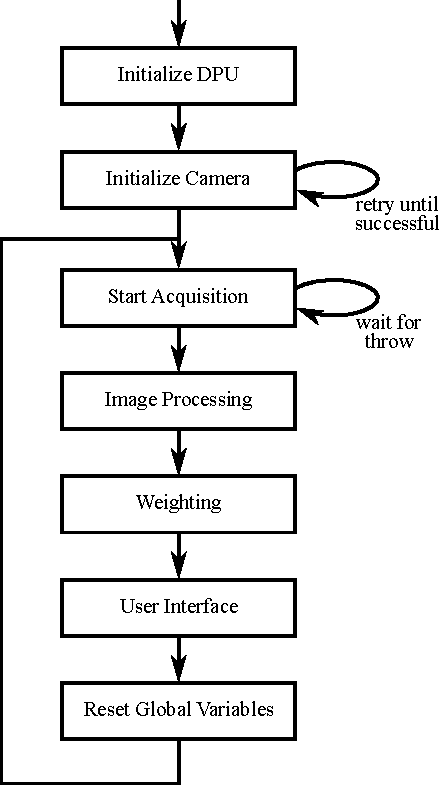
\includegraphics[width=0.5\textwidth]{program_flow}
  \caption{Procedure of the inference application}
  \label{fig:procedure_inference_app}
\end{figure}

% ------------------------------------------------------------------------------------------------------------------------------
\subsection{Initialization}
\label{subsec:inference:app:initialization}

The initialization process consists of two parts:
\begin{enumerate}
  \item Initializing the \acrshort{dpu}
  \item Initializing the camera
\end{enumerate}

% -----------------------------------------
\paragraph{Initializing the \acrshort{dpu}}
The initialization procedure of the \acrshort{dpu} consists of loading and setting up the \acrshort{dpu}.
This is done with the two Python packages \texttt{pynq\_dpu} and \texttt{dnndk}.
The \texttt{pynq\_dpu} package provides a class to load the desired \acrshort{dpu}.
The \texttt{dnndk} package contains the \texttt{n2cube} module, which is a thin wrapper around the \acrshort{n2cube} library and allows to interface with the implemented \acrshort{dpu} \cite{inf_github_dpu_pynq}.

The first step consists of loading the \acrshort{dpu} with the three overlay files \texttt{dpu.bit}, \texttt{dpu.hwh} and \texttt{dpu.xclbin}.
These files contain the bitstream to flash the \acrshort{dpu} to the \acrlong{pl} and the necessary information to interface with it.

The second step is to set up the \acrshort{dpu}.
Therefore, the \acrshort{n2cube} function \texttt{n2cube.dpuLoadKernel} is used to load a so-called kernel.
This kernel contains the architecture and the weights of the quantized \acrshort{cnn} model.

% ---------------------------------
\paragraph{Initializing the Camera}
To initialize the camera, the camera library has to be loaded first.
This is done with the Python package \texttt{ctypes}, which provides C compatible data types and allows to call functions of shared libraries \cite{inf_ctypes}.
Once loaded, the various mutator functions of the camera library are used to control settings such as the frame rate and the exposure time (see section \ref{sec:inference:camera_library}).

Finally, the camera is initialized by calling the function \texttt{libcamera.initialize}.
The return code of this function is used to check, whether the initialization was successful.
If an initialization error occurs, an error message is shown on the bootsplash screen.
The initialization function is called until it succeeds, which is listed in appendix \ref{app:inference_application} on lines \ref{lst:ln:camera_init1}--\ref{lst:ln:camera_init2}
This is to avoid a reboot of the entire system if the camera is not plugged in during the startup of the application.

% ------------------------------------------------------------------------------------------------------------------------------
\subsection{Image Acquisition}
\label{subsec:inference:app:image_acquisition}

The camera library features several accessor functions to access the global variables.
This enables the use of parallel processing.

The Python interpreter features a \acrfull{gil}, which allows only one thread to execute code \cite{inf_gil}.
However, the Python standard library contains two packages to realize thread-based and process-based parallelism.
On the one hand, thread-based parallelism can be realized with the \texttt{threading} package \cite{inf_threading}.
On the other hand, process-based parallelism can be realized with the \texttt{multiprocessing} package, which spawns a new process for each task \cite{inf_multiprocessing}.
Different threads run concurrently, which means that different tasks are executed at the same time, but not simultaneously.
Different processes can run simultaneously on different cores of the processor \cite{inf_parallelism}.

The problem with the \texttt{multiprocessing} package is, that different processes do not share memory.
This makes it impossible to poll the global variables, and therefore, the image processing can only begin after the image acquisition is complete.

Fortunately, in this case the \texttt{threading} package is ideal.
The \texttt{ctypes} package releases the \acrshort{gil} before calling a C function \cite{inf_ctypes_gil}.
This allows the \texttt{libcamera.start\_acquisition} function to run simultaneously in a thread on another processor core.

However, practical tests have shown that the embedded system is not powerful enough to acquire and process frames at the same time.
The camera library starts to drop frames as soon as another processor-intensive task, such as the image processing, is started.

Nevertheless, using a thread-based approach is still beneficial.
This is due to the specific implementation of the \texttt{libcamera.start\_acquisition} function, which introduces some overhead.
After a throw has ended, the function stops the device and the datastream before returning.
This task is not computationally intensive, but still requires a significant amount of time.

Therefore, the implementation of the image acquisition uses a thread and polls the global variable \texttt{throw\_end}.
As soon as the global variable \texttt{throw\_end} is set to \texttt{true}, the image processing begins.
This is shown in appendix \ref{app:inference_application} on lines \ref{lst:ln:threading}--\ref{lst:ln:polling}.

As soon as the image processing is done, the \texttt{libcamera.reset\_global\_variables} function is called to reset the global variables.
After that, the image acquisition and the polling of the global variable \texttt{throw\_end} is restarted.

% ------------------------------------------------------------------------------------------------------------------------------
\subsection{Image Processing}
\label{subsec:inference:app:image_processing}

The image classification chain consists of five serialized steps:

\begin{enumerate}
  \item Getting the raw Baumer \texttt{BayerRG8} frame
  \item Converting the color space
  \item Resizing the frame
  \item Normalizing the pixel values
  \item Running inference
\end{enumerate}

Steps one to four serve for image preprocessing and step five for the actual image classification.

However, it makes no sense to evaluate all frames of a throw, as this would strongly impact the total required classification time.
Furthermore, the classification accuracy of the \acrshort{cnn} model is quite high, so that a small number of frames is sufficient to make an accurate prediction.

Analysing the dataset reveals the ideal number of frames to consider, to cover all frames of at least \SI{80}{\percent} of all throws.
The empirical distribution of the number of frames per throw $f(x)$ is shown in figure \ref{fig:distribution}.
This distribution is used to derive the empirical cumulative distribution function $F(x)$ shown in figure \ref{fig:cumulative_distribution}.
It shows that \SI{80}{\percent} of all throws consist of \num{22} frames or less.
For this reason, a maximum of \num{22} frames are processed by the image classification chain.

\begin{figure}
  \centering
  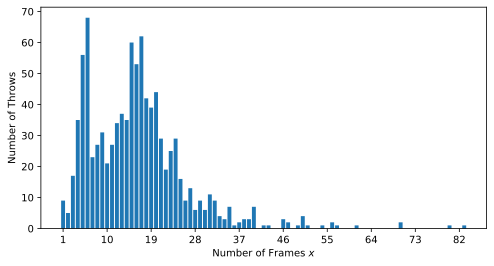
\includegraphics[width=\textwidth]{distribution}
  \caption{Distribution of the number of frames per throw $f(x)$}
  \label{fig:distribution}
\end{figure}

\begin{figure}
  \centering
  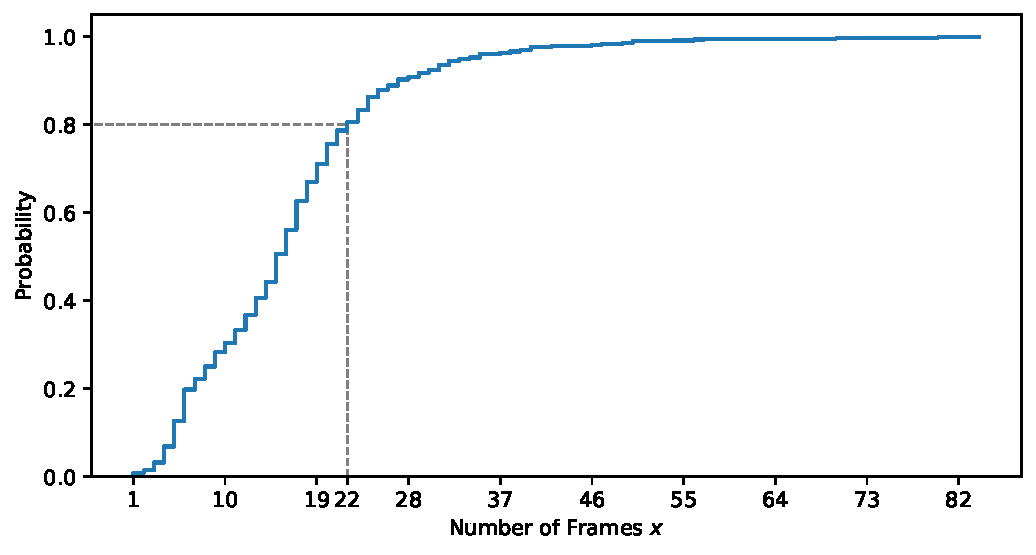
\includegraphics[width=\textwidth]{cumulative_distribution}
  \caption{Empirical cumulative distribution function $F(x)$}
  \label{fig:cumulative_distribution}
\end{figure}

% -----------------------------
\paragraph{Image Preprocessing}
The image preprocessing is is listed in appendix \ref{app:inference_application} on lines \ref{lst:ln:image_preprocessing1}--\ref{lst:ln:image_preprocessing2}.
For this purpose the Python packages NumPy and \acrshort{opencv} are used.
Those packages are just thin Python wrappers around the native-implemented libraries and therefore very performant.

The first step consists of getting the raw Baumer \texttt{BayerRG8} frame from memory and store it in a NumPy array.
This is done with the help of a pointer to the raw frame.

In a second step, the color space is converted from raw Baumer \texttt{BayerRG8} to \acrshort{bgr}.
The conversion uses the \acrshort{opencv} function \texttt{cvtColor}, which operates on NumPy arrays.
The required color space conversion code is set to \texttt{cv2.COLOR\_BayerBG2BGR} \cite{inf_opencv_color}.
This odd conversion code results from the fact that Baumer and \acrshort{opencv} use different naming schemes.
The Baumer \texttt{BayerRG} format corresponds to the \acrshort{opencv} \texttt{BayerBG} format.

The third step is to resize the frames with the \acrshort{opencv} function \texttt{cv2.resize}.
This function is supplied with three arguments: the NumPy array that represents the image, the desired output image size and the interpolation method \cite{training_opencv_resize}.
For performance reasons, the nearest-neighbor interpolation method is used (see section \ref{subsec:training_of_the_cnn:dataset:augmentation}).

The last step consists of normalizing the individual pixel values to the range between \numrange{0}{1}, just as it was done during training (see section \ref{sec:training_of_the_cnn:training}).

% ------------------------------
\paragraph{Image Classification}
The actual image classification is done with the \acrshort{n2cube} function \texttt{n2cube.dpuRunTask}, which uses the quantized \acrshort{cnn} model to make a prediction on the supplied input image.
This is shown in appendix \ref{app:inference_application} on line \ref{lst:ln:image_classification}.

The output values of the quantized \acrshort{cnn} model are denoted by the output vector

\begin{equation}
  \boldsymbol{z} =
  \begin{bmatrix}
    z_1 & z_2 & \dots & z_c \\
  \end{bmatrix}.
  \label{eq:output_vector}
\end{equation}

The values of the output vector $\boldsymbol{z}$ are 8-bit signed integers which represent a fixed-point format.
To normalize the values of the output vector to a discrete probability distribution over the target classes, the softmax function is used \cite{inf_softmax}.
Calculating the individual probabilities is done with equation \ref{eq:softmax}.

\begin{equation}
  p_k = \frac{e^{z_k}}{\sum\limits_{i=1}^{c} e^{z_i}}
  \label{eq:softmax}
\end{equation}

where

\[
  k = 1, 2, \dots, c
\]

and

\begin{tabular}{lll}
  $p_k$ & = & probability $k$ of the prediction vector $\boldsymbol{p}$ \\
  $z_k$ & = & output value $k$ of output vector $\boldsymbol{z}$ \\
  $c$ & = & number of classes \\
  $z_i$ & = & output value $i$ of output vector $\boldsymbol{z}$ \\
\end{tabular}
\\

The softmax function is implemented with the \acrshort{n2cube} function \texttt{n2cube.dpuRunSoftmax}, which returns the prediction vector in the form of a NumPy array.
Whenever a probability is equal to \num{1.0}, the \acrshort{n2cube} softmax function returns \texttt{NaN} at the respective position.
The reason for this could be that the fixed-point format used is not capable of representing a \num{1.0}.
Therefore, a code section in the Python script replaces the first occurance of \texttt{NaN} with a probability of \num{1.0}.
The softmax implementation is shown in appendix \ref{app:inference_application} on lines \ref{lst:ln:softmax1}--\ref{lst:ln:softmax2}.

This results in the prediction vector

\begin{equation}
  \boldsymbol{p} =
  \begin{bmatrix}
    p_1 & p_2 & \dots & p_c \\
  \end{bmatrix}.
  \label{eq:prediction_vector}
\end{equation}

The individual prediction vectors of the individual frames are then combined to a column vector, which results in the predictions matrix $\boldsymbol{P}$ shown in equation \ref{eq:predictions_matrix}.
The predictions matrix is implemented as a two-dimensional NumPy array shown in appendix \ref{app:inference_application} on line \ref{lst:ln:predictions_matrix}.

\begin{equation}
  \boldsymbol{P} =
  \begin{bmatrix}
    \boldsymbol{p}_1 \\
    \boldsymbol{p}_2 \\
    \vdots \\
    \boldsymbol{p}_n \\
  \end{bmatrix} =
  \begin{bmatrix}
    P_{11} & P_{12} & \dots & P_{1c} \\
    P_{21} & P_{22} & \dots & P_{2c} \\
    \vdots & \vdots & \ddots & \vdots \\
    P_{n1} & P_{n2} & \dots & P_{nc} \\
  \end{bmatrix}
  \label{eq:predictions_matrix}
\end{equation}

% ------------------------------------------------------------------------------------------------------------------------------
\subsection{Weighting}
\label{subsec:inference:app:weighting}

Verifying the classification accuracy has shown that images in which the object is fully visible perform significantly better than frames in which the object is only partially visible (see section \ref{subsec:verification_and_benchmark:classification_performance:inference}).
For this reason, a discrete sine-squared weighting function is applied to the predictions.

% --------------------------
\paragraph{Number of Frames}
To properly weight the predictions, not only the number of frames considered $n$ is important, but also the total number of frames $N$.
The relationship between the two is given in equation \ref{eq:number_of_frames}.
Not considering the total number of frames would implicitly assume that the throw was only \num{22} frames long.
Throws of larger objects, which generally create more frames, would then be incorrectly weighted.
Furthermore, knowing if the throw created more than \num{44} frames is not really beneficial because of the symmetry of the weighting function.
This information would only be relevant if the total number of frames could get extremely large, which it cannot.

\begin{equation}
  n =
  \begin{cases}
    N & N \leq 22 \\
    22 & N > 22 \\
  \end{cases}
  \label{eq:number_of_frames}
\end{equation}

where

\begin{tabular}{lll}
  $n$ & = & number of frames considered \\
  $N$ & = & total number of frames \\
\end{tabular}
\\

% ----------------------------
\paragraph{Weighting Function}
The used weighting function is the discrete version of a stretched and phase-shifted sine-squared window function.
The individual weights can be calculated with equation \ref{eq:weighting_function}.
An example of the discrete weighting function with $n = 22$ and $N = 28$ is shown in figure \ref{fig:weighting_function}.

\begin{equation}
  w_k = \sin^2\left(\frac{k}{N+1} \cdot \pi \right)
  \label{eq:weighting_function}
\end{equation}

where

\[
  k = 1, 2, \dots, n
\]

and

\begin{tabular}{lll}
  $w_k$ & = & weighting factor $k$ of the weight vector $\boldsymbol{w}$ \\
  $N$ & = & total number of frames \\
  $n$ & = & number of frames considered \\
\end{tabular}
\\

\begin{figure}
  \centering
  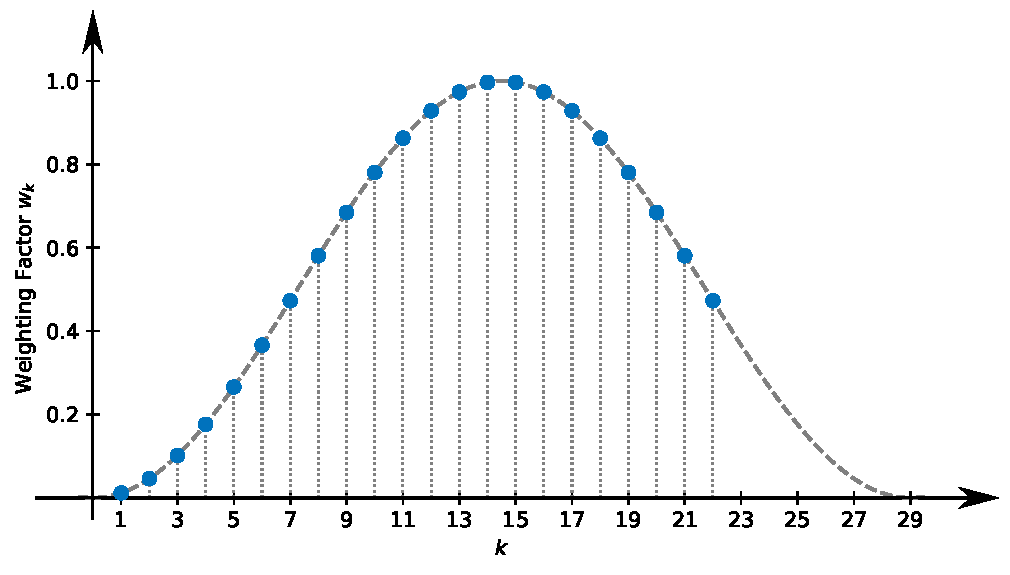
\includegraphics[width=\textwidth]{weighting_function}
  \caption{Weighting function with $n = 22$ and $N = 28$}
  \label{fig:weighting_function}
\end{figure}

This results in the weight vector
\begin{equation}
  \boldsymbol{w} =
  \begin{bmatrix}
    w_{1} & w_{2} & \dots & w_{n} \\
  \end{bmatrix}.
  \label{eq:weight_vector}
\end{equation}

The weight vector is implemented as a fixed size one-dimensional NumPy array.
The length of this array corresponds to the maximum number of frames to be considered, which is \num{22}.
If a throw creates less than \num{22} frames, the rest of the array is filled with zeros.
This is implemented in the \texttt{sine\_squared\_window} function, as shown in appendix \ref{app:inference_application} on line \ref{lst:ln:sine_squared_window}.

% --------------------------------------
\paragraph{Weighting of the Predictions} % Probabilities
The individual probabilities are weighted according to equation \ref{eq:weighted_probability}.

\begin{equation}
  y_k = \frac{w_1 \cdot P_{1k} + w_2 \cdot P_{2k} + \dots + w_n \cdot P_{nk}}{w_1 + w_2 + \dots + w_n} = \frac{\sum\limits_{i=1}^{n} w_i \cdot P_{ik}}{\sum\limits_{i=1}^{n} w_i}
  \label{eq:weighted_probability}
\end{equation}

where

\[
  k = 1, 2, \dots, c
\]

and

\begin{tabular}{lll}
  $y_k$ & = & weighted probability $k$ of the weighted prediction vector $\boldsymbol{y}$ \\
  $w_i$ & = & weighting factor $i$ of the weight vector $\boldsymbol{w}$ \\
  $P_{i,k}$ & = & probability $i,k$ of the predictions matrix $\boldsymbol{P}$ \\
  $n$ & = & number of frames considered \\
  $c$ & = & number of classes \\
\end{tabular}
\\

This results in the weighted prediction vector
\begin{equation}
  \boldsymbol{y} =
  \begin{bmatrix}
    y_{1} & y_{2} & \dots & y_{n} \\
  \end{bmatrix}.
  \label{eq:weighted_prediction_vector}
\end{equation}

The actual implementation uses matrix multiplication to perform this calculation efficiently.
Therefore, the NumPy function \texttt{np.matmul} is used to calculate the matrix product of the two arrays \cite{inf_numpy_matmul}.
This is shown in appendix \ref{app:inference_application} on line \ref{lst:ln:matrix_multiplication}.

\begin{equation}
  \boldsymbol{y} = \sum\limits_{i=1}^{n} w_i^{-1} \cdot \boldsymbol{w} \boldsymbol{P}
  \label{eq:weighted_prediction}
\end{equation}

where

\begin{tabular}{lll}
  $\boldsymbol{y}$ & = & weighted prediction vector \\
  $n$ & = & number of frames considered \\
  $w_i$ & = & weighting factor $i$ of the weight vector $\boldsymbol{w}$ \\
  $\boldsymbol{w}$ & = & weight vector \\
  $\boldsymbol{P}$ & = & predictions matrix \\
\end{tabular}
\\

% ------------------------------------------------------------------------------------------------------------------------------
\subsection{User Interface}
\label{subsec:inference:app:ui}

The results must be prepared to be displayed on the screen.
On the one hand, an appropriate frame of the captured throw has to be selected and, on the other hand, the probabilities have to be rounded and prepared in a list.

% -------------------------
\paragraph{Frame Selection}
Choosing an appropriate frame of the captured throw is done by selecting the image with the highest weighted probability of the class selected as the best prediction.
For this purpose, the element-wise multiplication of the weight column vector $\boldsymbol{w}^\top$ with the respective column of the predictions matrix $\boldsymbol{P}$ is calculated.
This is shown in equation \ref{eq:weighted_probabilities}.
The image corresponding to the index of the highest weighted probability is then selected.
Due to the applied weighting, this is most likely a frame from the middle of the throw, where the object is most visible.

\begin{equation}
  \boldsymbol{f} = \boldsymbol{w}^\top \circ \boldsymbol{P}_{:,k} =
  \begin{bmatrix}
    w_{1} \cdot P_{1,k} \\
    w_{2} \cdot P_{2,k} \\
    \vdots \\
    w_{n} \cdot P_{n,k} \\
  \end{bmatrix}
  \label{eq:weighted_probabilities}
\end{equation}

where

\begin{tabular}{lll}
  $\boldsymbol{f}$ & = & weighted probabilities column vector \\
  $\boldsymbol{w}^\top$ & = & weight column vector \\
  $\boldsymbol{P}_{:,k}$ & = & column $k$ of the predictions matrix $\boldsymbol{P}$ \\
  $w_i$ & = & weighting factor $i$ of the weight vector $\boldsymbol{w}$ \\
  $P_{i,k}$ & = & probability $i,k$ of the predictions matrix $\boldsymbol{P}$ \\
  $n$ & = & number of frames considered \\
\end{tabular}
\\

The frame is then resized and encoded as a \acrshort{png}.
The implementation of the image selection and preparation process is shown in appendix \ref{app:inference_application} on lines \ref{lst:ln:frame_selection1}--\ref{lst:ln:frame_selection2}.

% ---------------------------------------
\paragraph{Rounding of the Probabilities}
The probabilities (in percent) are rounded to one decimal place before they are displayed on the screen.
However, naively rounding percentages will quickly reveal the problem that the total value does not always add up to \SI{100}{\percent}.
The largest remainder method is used to fix this problem.
This simple method consists of the following easy three steps \cite{inf_percentage}:
\begin{enumerate}
  \item Flooring all values
  \item Computing the difference between the total value and the sum of the floored values
  \item Distributing this difference by incrementing the floored values in decreasing order of their decimal parts
\end{enumerate}

The largest remainder method is implemented in the \texttt{lrm\_round} function, as shown in appendix \ref{app:inference_application} on line \ref{lst:ln:lrm_round}.
To round the percentages to one decimal place, the values are multiplied by ten before the algorithm is applied.
In a final step, the values are divided by ten, resulting in percentages rounded to one decimal place.
